% Add this in your LaTeX report preamble:
% \usepackage{graphicx}

\begin{figure}[t]
  \centering
  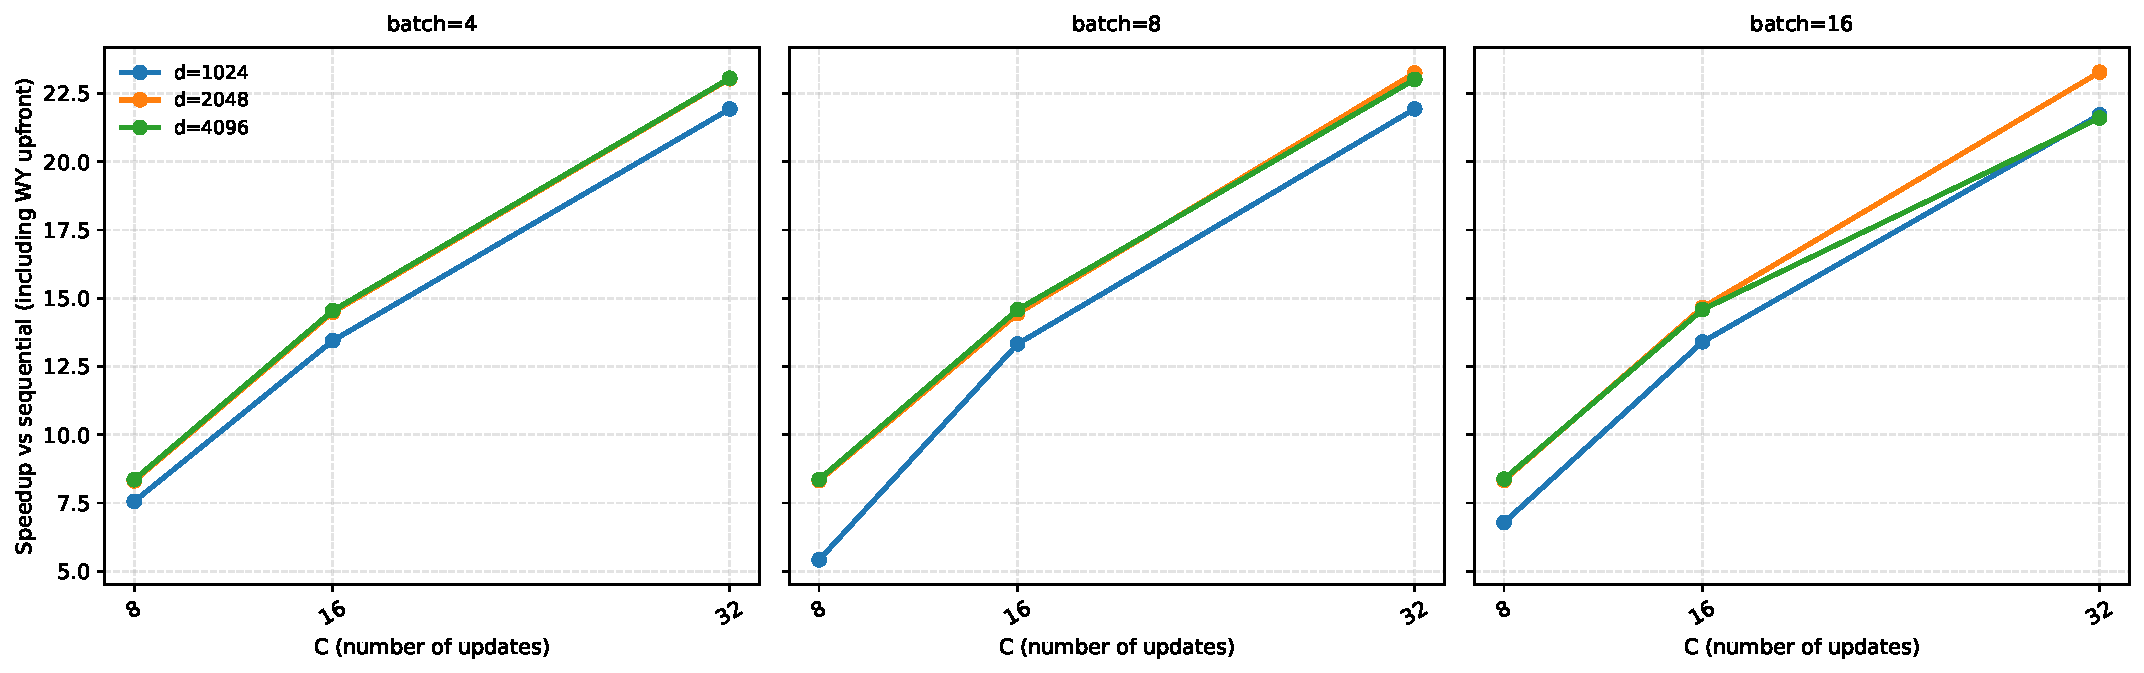
\includegraphics[width=\linewidth]{fig_speedup_vs_C.pdf}
  \caption{WY speedup (including amortized upfront build) as a function of C for each batch and d.}
  \label{fig:wy-speedup}
\end{figure}

\begin{figure}[t]
    \centering
    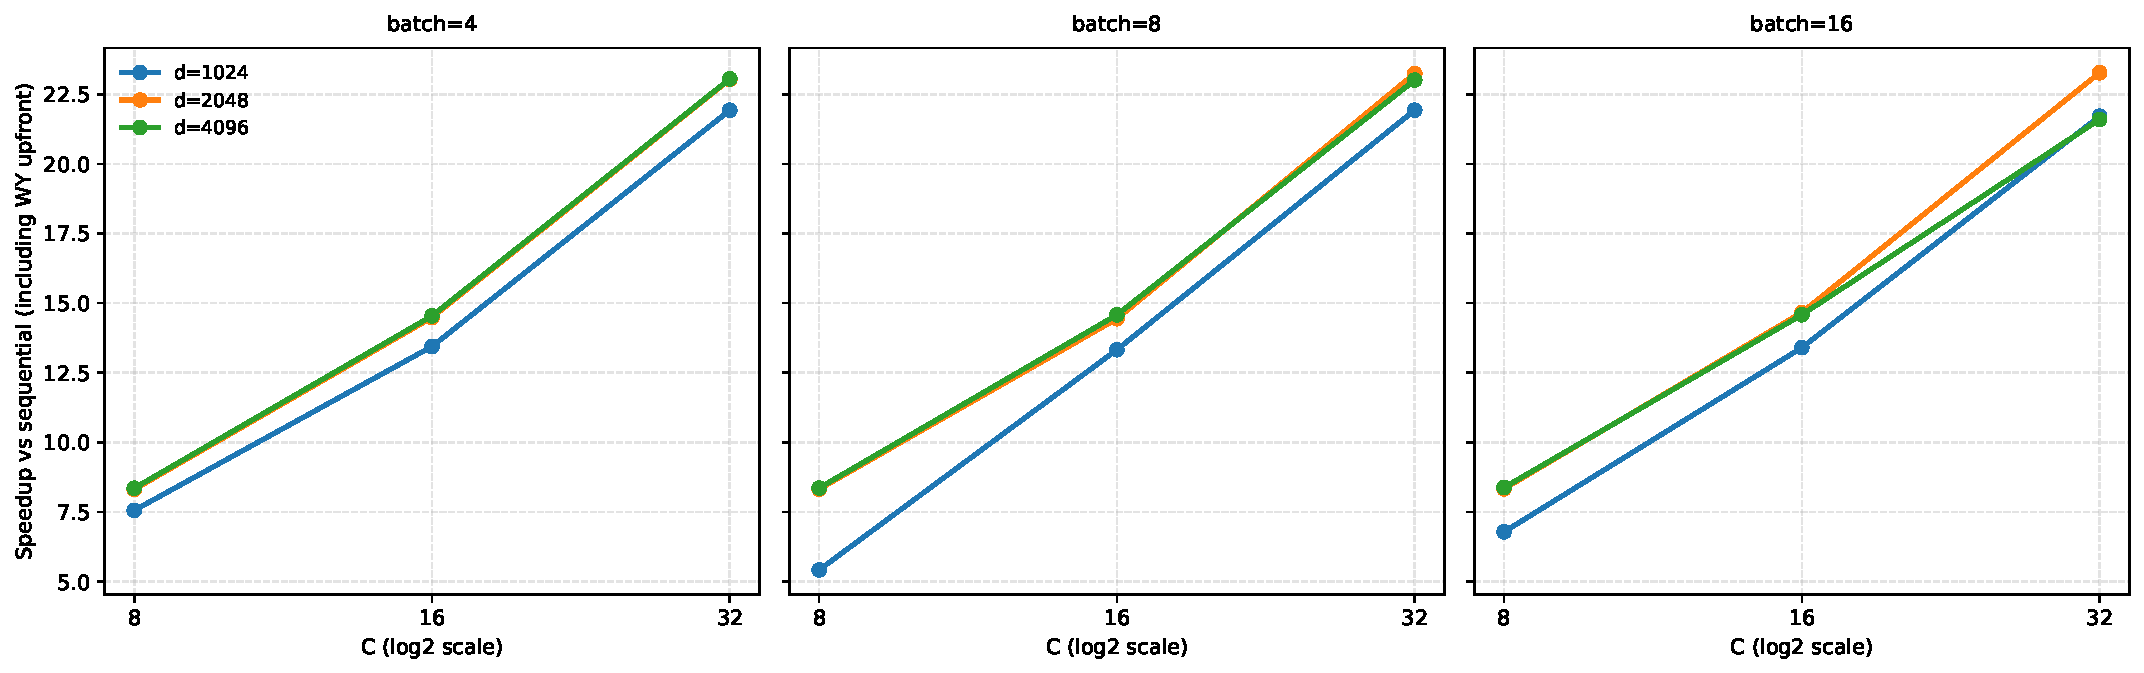
\includegraphics[width=\linewidth]{fig_speedup_vs_C_logx.pdf}
    \caption{Same speedup plot with a log2 x-axis for clearer comparison across small and large C.}
    \label{fig:wy-speedup-logx}
\end{figure}

\begin{figure}[t]
  \centering
  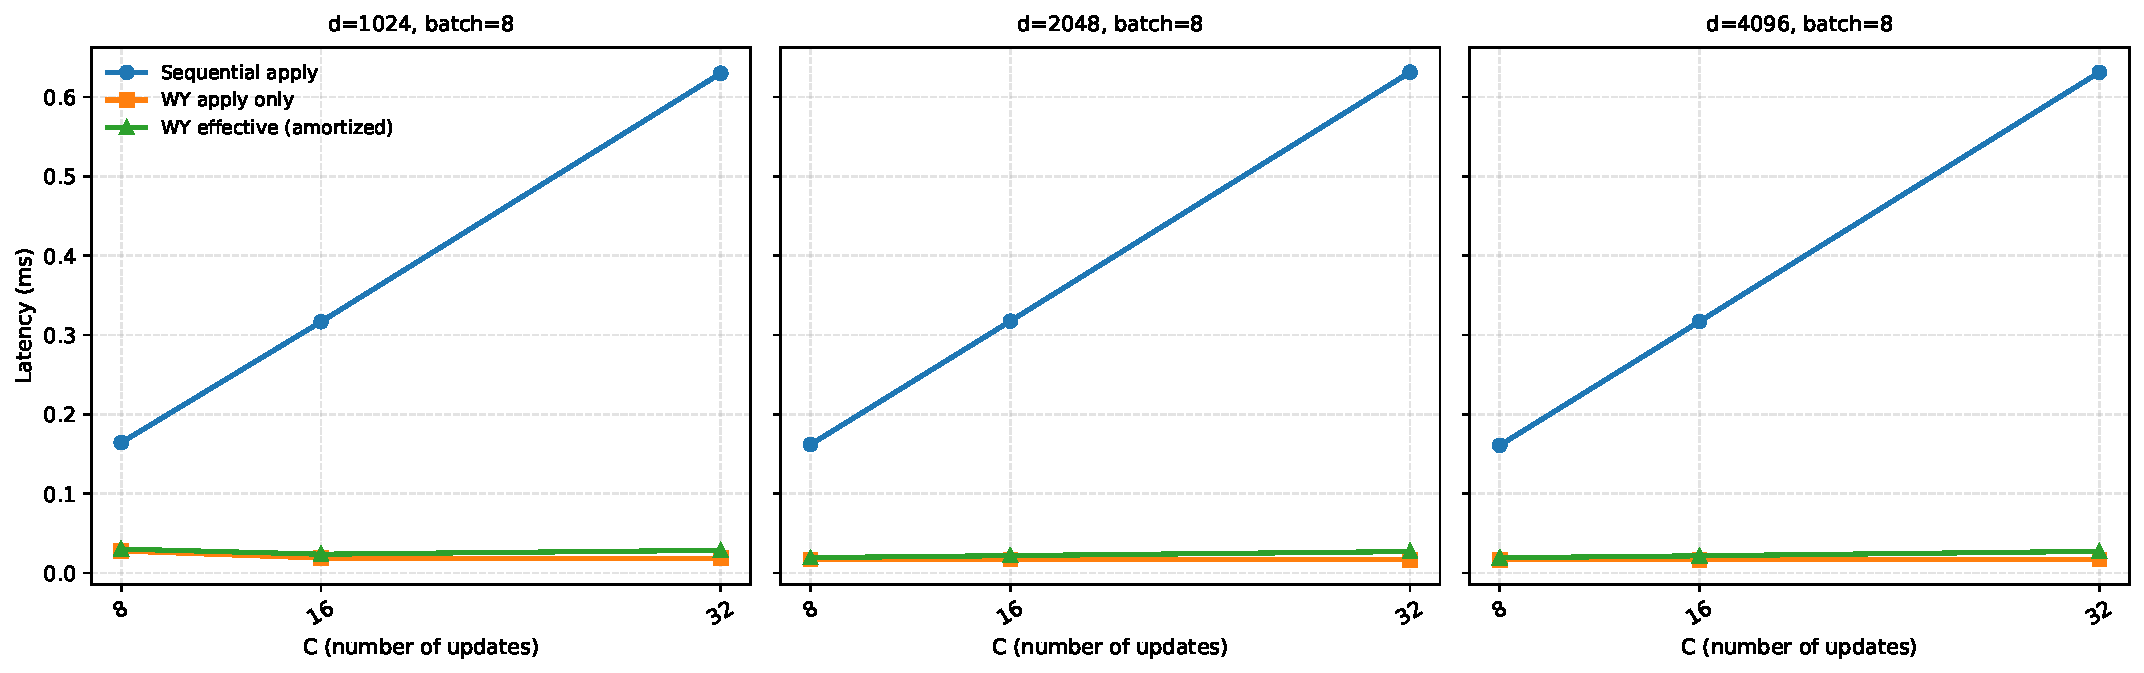
\includegraphics[width=\linewidth]{fig_latency_vs_C.pdf}
  \caption{Sequential vs WY apply latency, including effective WY latency with amortized upfront cost.}
  \label{fig:wy-latency}
\end{figure}

\begin{figure}[t]
  \centering
  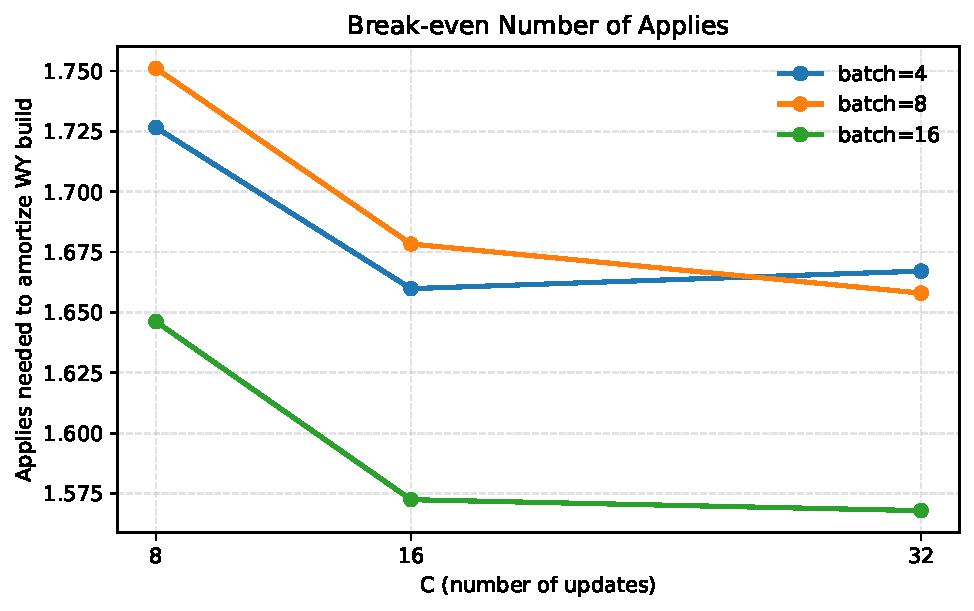
\includegraphics[width=0.8\linewidth]{fig_break_even.pdf}
  \caption{Break-even number of applies needed to amortize WY build cost.}
  \label{fig:wy-break-even}
\end{figure}
